\subsection{課題1}

ある一つの粒子について、原点を適当に定め座標を5秒ごとに記録した結果を表\ref{tab:position}に示す。
なお、座標の有効数字はソフトウェア上では\SI{1}{\nano\meter}のオーダーまで計測できていたが、光学顕微鏡の分解能はおおよそ光の波長程度であり、\SI{10}{\nano\meter}のオーダーを四捨五入し、\SI{100}{\nano\meter}のオーダーにした。
また、表\ref{tab:position}の$x_m$と$y_m$は、\SI{10}{\micro\meter}ごとに線が切られたマイクロメーターをソフトウェア上で5回計測した結果が表\ref{tab:micrometer}で、その平均が\SI{10.04}{\micro\meter}であったから、$x_m = x \times \dfrac{10}{10.04}$と$y_m = y \times \dfrac{10}{10.04}$として校正した値である。
$\Delta x_m$、$\Delta y_m$はそれぞれ$x_m$、$y_m$の差分である。
この $\Delta x_m$、$\Delta y_m$についてヒストグラムを作成すると、図\ref{fig:delta-x-y-histogram}のようになる。

\begin{longtable} {c}
    \caption{\SI{10}{\micro\meter}のソフトウェア上での計測結果} \label{tab:micrometer} \\
    \hline 距離 $d$ /\SI{}{\micro\meter}                                   \\ \hline
    \endfirsthead

    \hline
    \endlastfoot
    9.9                                                                  \\
    9.9                                                                  \\
    10                                                                   \\
    10.2                                                                 \\
    10.2                                                                 \\
\end{longtable}

\newpage
\begin{longtable}{ccccccc}
    \caption{粒子の座標} \label{tab:position}                                                                                                                                                                               \\
    \hline 時間 $T$ /\SI{}{\sec} & $x$ /\SI{}{\micro\meter} & $y$ /\SI{}{\micro\meter} & $x_m$ /\SI{}{\micro\meter} & $y_m$ /\SI{}{\micro\meter} & $\Delta x_m$ /\SI{}{\micro\meter} & $\Delta y$ /\SI{}{\micro\meter}   \\ \hline
    \endfirsthead
    \hline 時間 $T$ /\SI{}{\sec} & $x$ /\SI{}{\micro\meter} & $y$ /\SI{}{\micro\meter} & $x_m$ /\SI{}{\micro\meter} & $y_m$ /\SI{}{\micro\meter} & $\Delta x$ /\SI{}{\micro\meter}   & $\Delta y_m$ /\SI{}{\micro\meter} \\ \hline
    \endhead
    \hline \multicolumn{7}{r}{次のページへ続く。}                                                                                                                                                                               \\ \hline
    \endfoot
    \hline
    \endlastfoot
    0                          & 71.2                     & 60.8                     & 70.9                       & 60.6                       & -                                 & -                                 \\
    5                          & 72.0                     & 59.1                     & 71.7                       & 58.8                       & 0.8                               & -1.8                              \\
    10                         & 69.7                     & 58.5                     & 69.4                       & 58.3                       & -2.3                              & -0.6                              \\
    15                         & 68.7                     & 56.6                     & 68.4                       & 56.4                       & -1.0                              & -1.9                              \\
    20                         & 69.1                     & 54.3                     & 68.8                       & 54.1                       & 0.4                               & -2.3                              \\
    25                         & 67.2                     & 53.9                     & 66.9                       & 53.7                       & -1.9                              & -0.4                              \\
    30                         & 64.0                     & 53.5                     & 63.7                       & 53.2                       & -3.2                              & -0.5                              \\
    35                         & 64.7                     & 52.8                     & 64.4                       & 52.6                       & 0.7                               & -0.7                              \\
    40                         & 63.7                     & 53.4                     & 63.4                       & 53.1                       & -1.0                              & 0.6                               \\
    45                         & 63.2                     & 53.4                     & 62.9                       & 53.1                       & -0.5                              & 0.0                               \\
    50                         & 61.4                     & 53.3                     & 61.2                       & 53.1                       & -1.8                              & -0.1                              \\
    55                         & 60.1                     & 51.5                     & 59.9                       & 51.3                       & -1.3                              & -1.8                              \\
    60                         & 59.2                     & 51.4                     & 59.0                       & 51.2                       & -0.9                              & -0.1                              \\
    65                         & 56.1                     & 49.3                     & 55.9                       & 49.1                       & -3.1                              & -2.0                              \\
    70                         & 53.6                     & 49.6                     & 53.4                       & 49.4                       & -2.5                              & 0.3                               \\
    75                         & 52.8                     & 48.1                     & 52.6                       & 47.9                       & -0.8                              & -1.5                              \\
    80                         & 53.5                     & 47.0                     & 53.3                       & 46.8                       & 0.7                               & -1.1                              \\
    85                         & 53.1                     & 46.4                     & 52.9                       & 46.3                       & -0.4                              & -0.6                              \\
    90                         & 53.8                     & 44.2                     & 53.6                       & 44.0                       & 0.7                               & -2.2                              \\
    95                         & 51.7                     & 41.3                     & 51.5                       & 41.1                       & -2.1                              & -2.9                              \\
    100                        & 50.4                     & 42.2                     & 50.2                       & 42.1                       & -1.3                              & 0.9                               \\
    105                        & 47.8                     & 40.7                     & 47.6                       & 40.5                       & -2.6                              & -1.6                              \\
    110                        & 46.3                     & 36.9                     & 46.1                       & 36.8                       & -1.5                              & -3.7                              \\
    115                        & 42.0                     & 35.7                     & 41.8                       & 35.6                       & -4.3                              & -1.2                              \\
    120                        & 40.1                     & 35.9                     & 39.9                       & 35.7                       & -1.9                              & 0.2                               \\
    125                        & 36.4                     & 35.6                     & 36.3                       & 35.5                       & -3.7                              & -0.3                              \\
    130                        & 34.5                     & 34.7                     & 34.4                       & 34.5                       & -1.9                              & -0.9                              \\
    135                        & 31.9                     & 32.7                     & 31.8                       & 32.6                       & -2.6                              & -2.0                              \\
    140                        & 32.4                     & 30.7                     & 32.3                       & 30.5                       & 0.5                               & -2.0                              \\
    145                        & 31.9                     & 31.0                     & 31.8                       & 30.9                       & -0.5                              & 0.4                               \\
    150                        & 31.0                     & 29.8                     & 30.9                       & 29.7                       & -0.9                              & -1.2                              \\
    155                        & 30.2                     & 29.1                     & 30.1                       & 28.9                       & -0.8                              & -0.7                              \\
    160                        & 29.3                     & 27.0                     & 29.2                       & 26.9                       & -0.9                              & -2.0                              \\
    165                        & 24.6                     & 24.7                     & 24.5                       & 24.6                       & -4.7                              & -2.3                              \\
    170                        & 23.9                     & 22.1                     & 23.8                       & 22.1                       & -0.7                              & -2.5                              \\
    175                        & 22.0                     & 21.4                     & 21.9                       & 21.3                       & -1.9                              & -0.7                              \\
    180                        & 20.4                     & 21.0                     & 20.3                       & 20.9                       & -1.6                              & -0.4                              \\
    185                        & 18.4                     & 21.3                     & 18.3                       & 21.2                       & -2.0                              & 0.3                               \\
    190                        & 20.1                     & 19.5                     & 20.0                       & 19.5                       & 1.7                               & -1.8                              \\
    195                        & 20.6                     & 16.8                     & 20.5                       & 16.8                       & 0.5                               & -2.7                              \\
    200                        & 18.6                     & 14.9                     & 18.5                       & 14.8                       & -2.0                              & -2.0                              \\
    205                        & 14.7                     & 12.9                     & 14.6                       & 12.8                       & -3.9                              & -2.0                              \\
    210                        & 14.5                     & 13.8                     & 14.4                       & 13.8                       & -0.2                              & 0.9                               \\
    215                        & 13.2                     & 11.3                     & 13.1                       & 11.3                       & -1.3                              & -2.5                              \\
    220                        & 10.3                     & 9.2                      & 10.3                       & 9.1                        & -2.9                              & -2.1                              \\
    225                        & 8.2                      & 6.8                      & 8.2                        & 6.8                        & -2.1                              & -2.3                              \\
    230                        & 8.2                      & 7.8                      & 8.2                        & 7.7                        & 0.0                               & 0.9                               \\
    235                        & 7.3                      & 6.4                      & 7.3                        & 6.3                        & -0.9                              & -1.4                              \\
    240                        & 4.3                      & 5.0                      & 4.3                        & 4.9                        & -3.0                              & -1.4                              \\
    245                        & 2.0                      & 5.1                      & 2.0                        & 5.1                        & -2.3                              & 0.2                               \\
    250                        & 2.0                      & 3.7                      & 2.0                        & 3.7                        & 0.0                               & -1.4                              \\
\end{longtable}


\newpage
\begin{figure}[htbp]
    \centering
    \begin{minipage}[b]{0.45\linewidth}
        \centering
        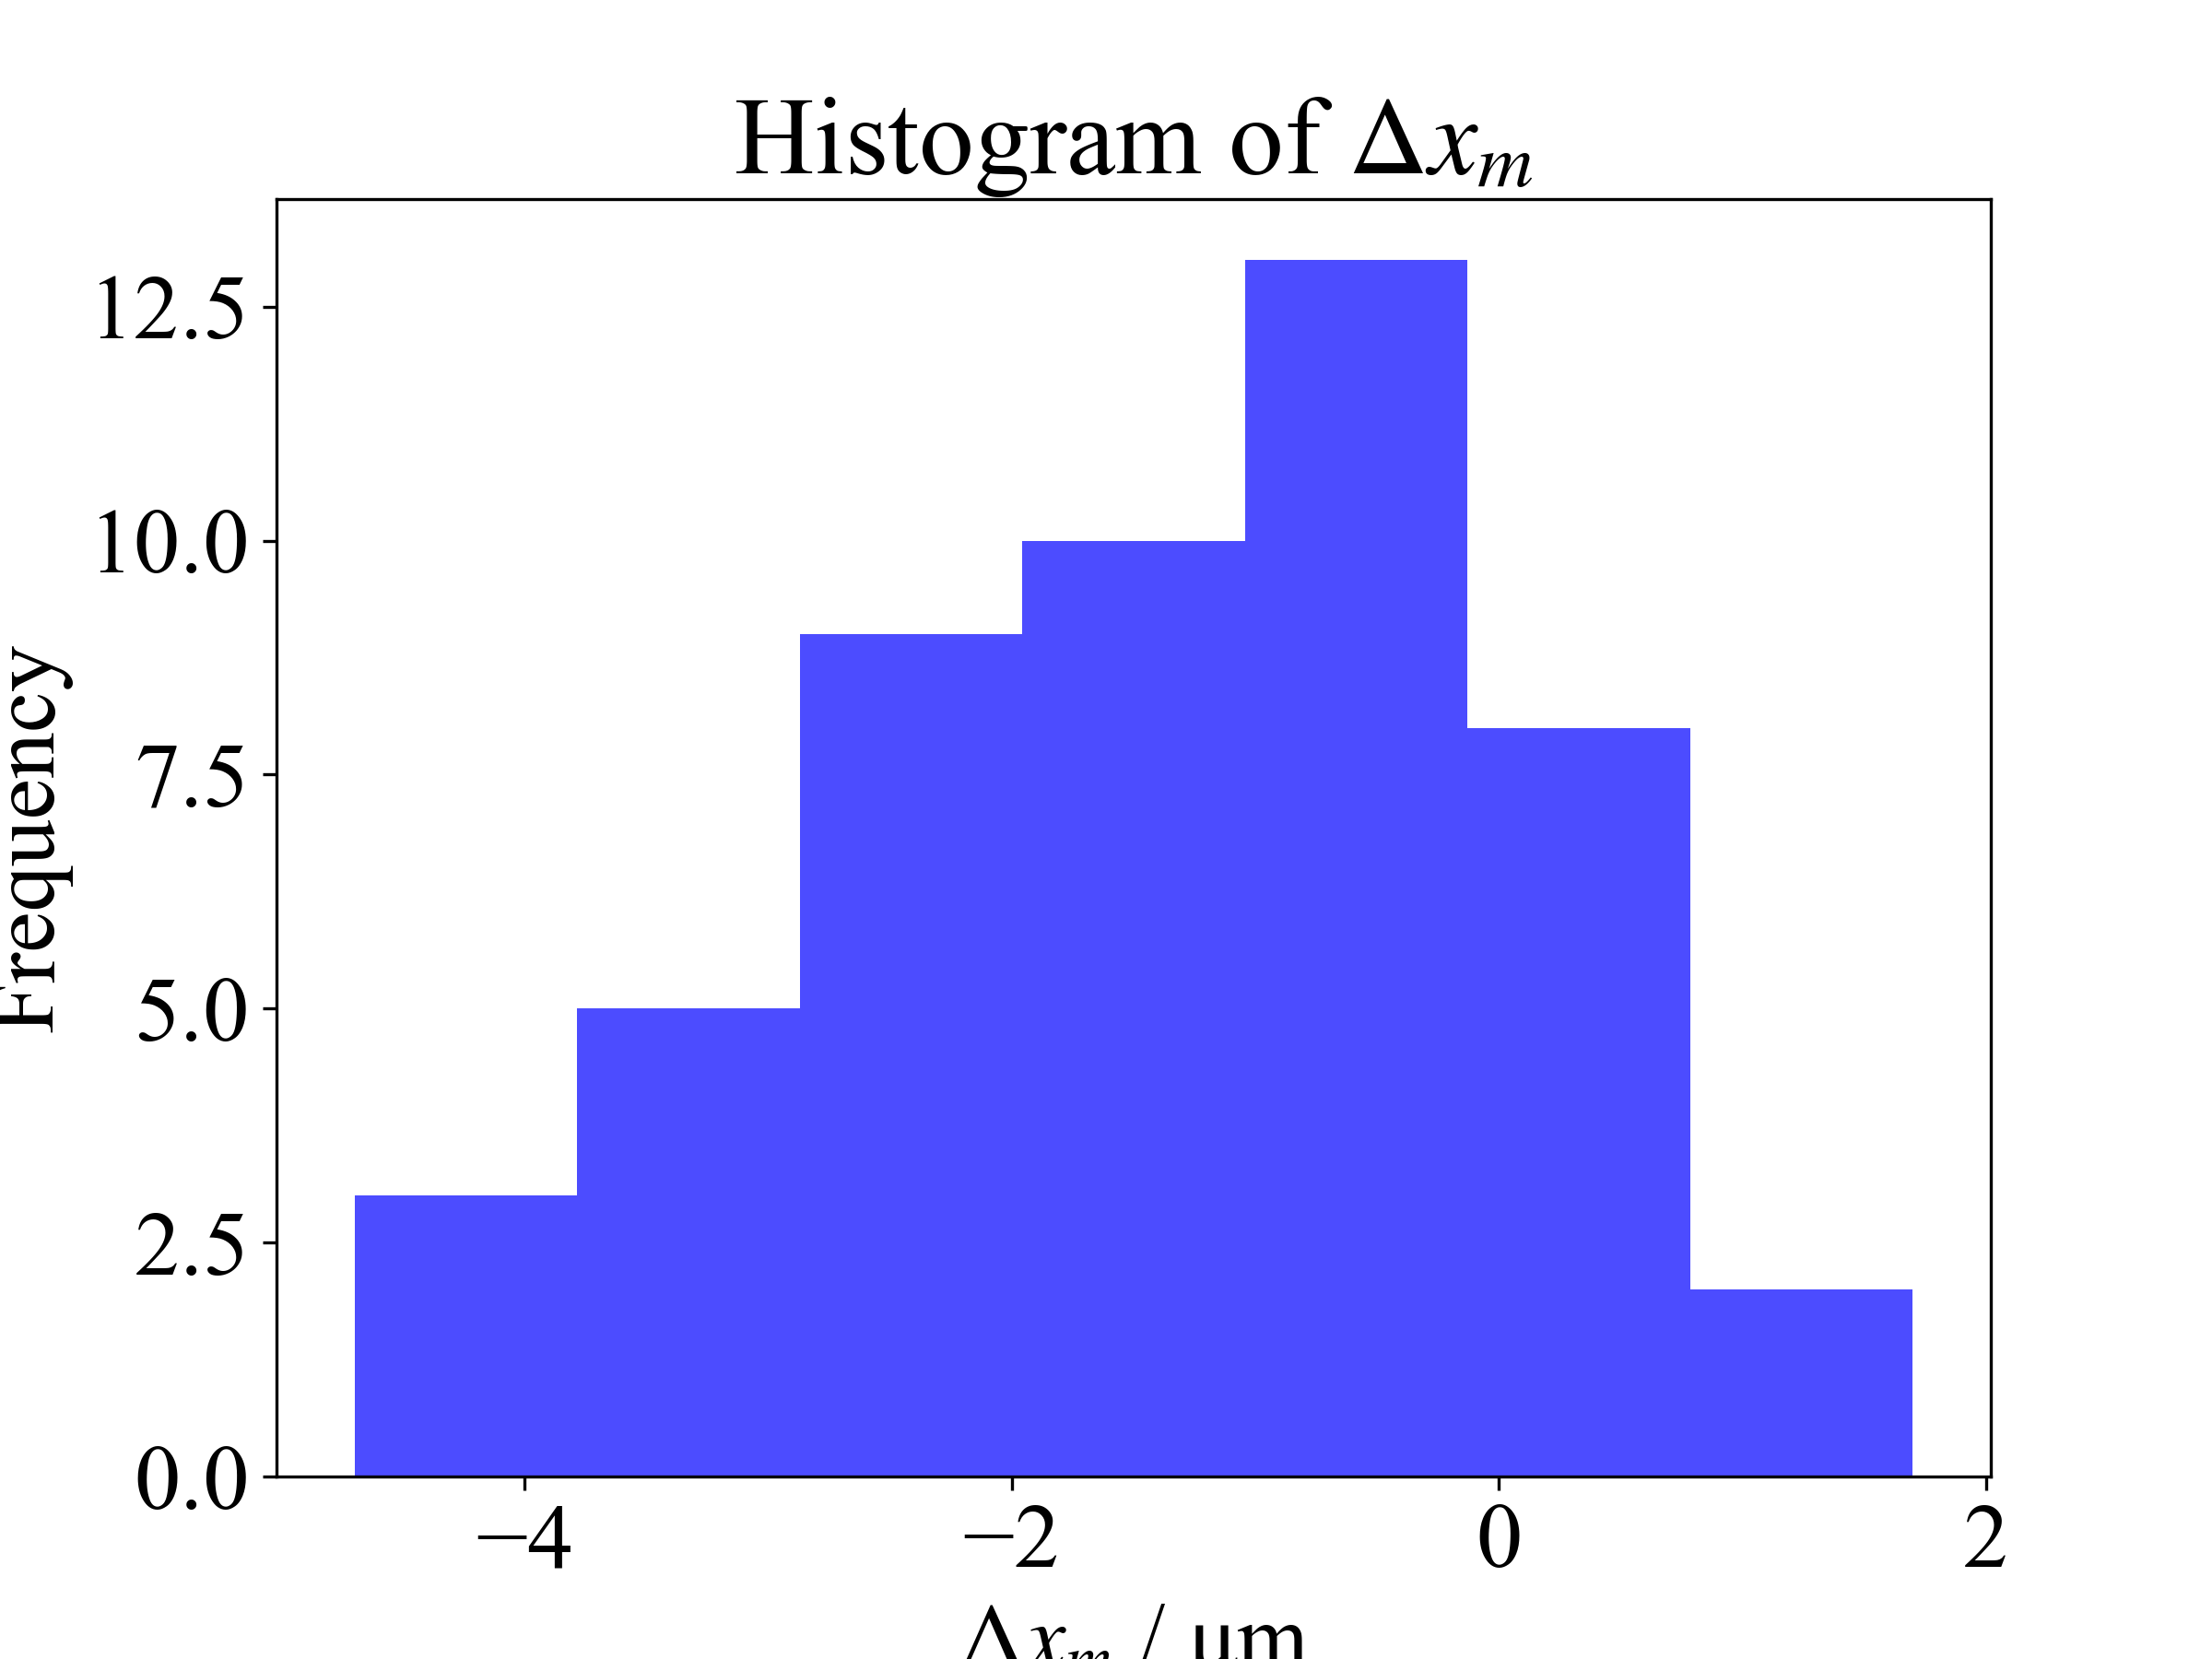
\includegraphics[keepaspectratio, width=\linewidth]{src/figures/delta-x-y-histogram/delta-x-histogram.png}
        \subcaption{$\Delta x_m$}
    \end{minipage}
    \begin{minipage}[b]{0.45\linewidth}
        \centering
        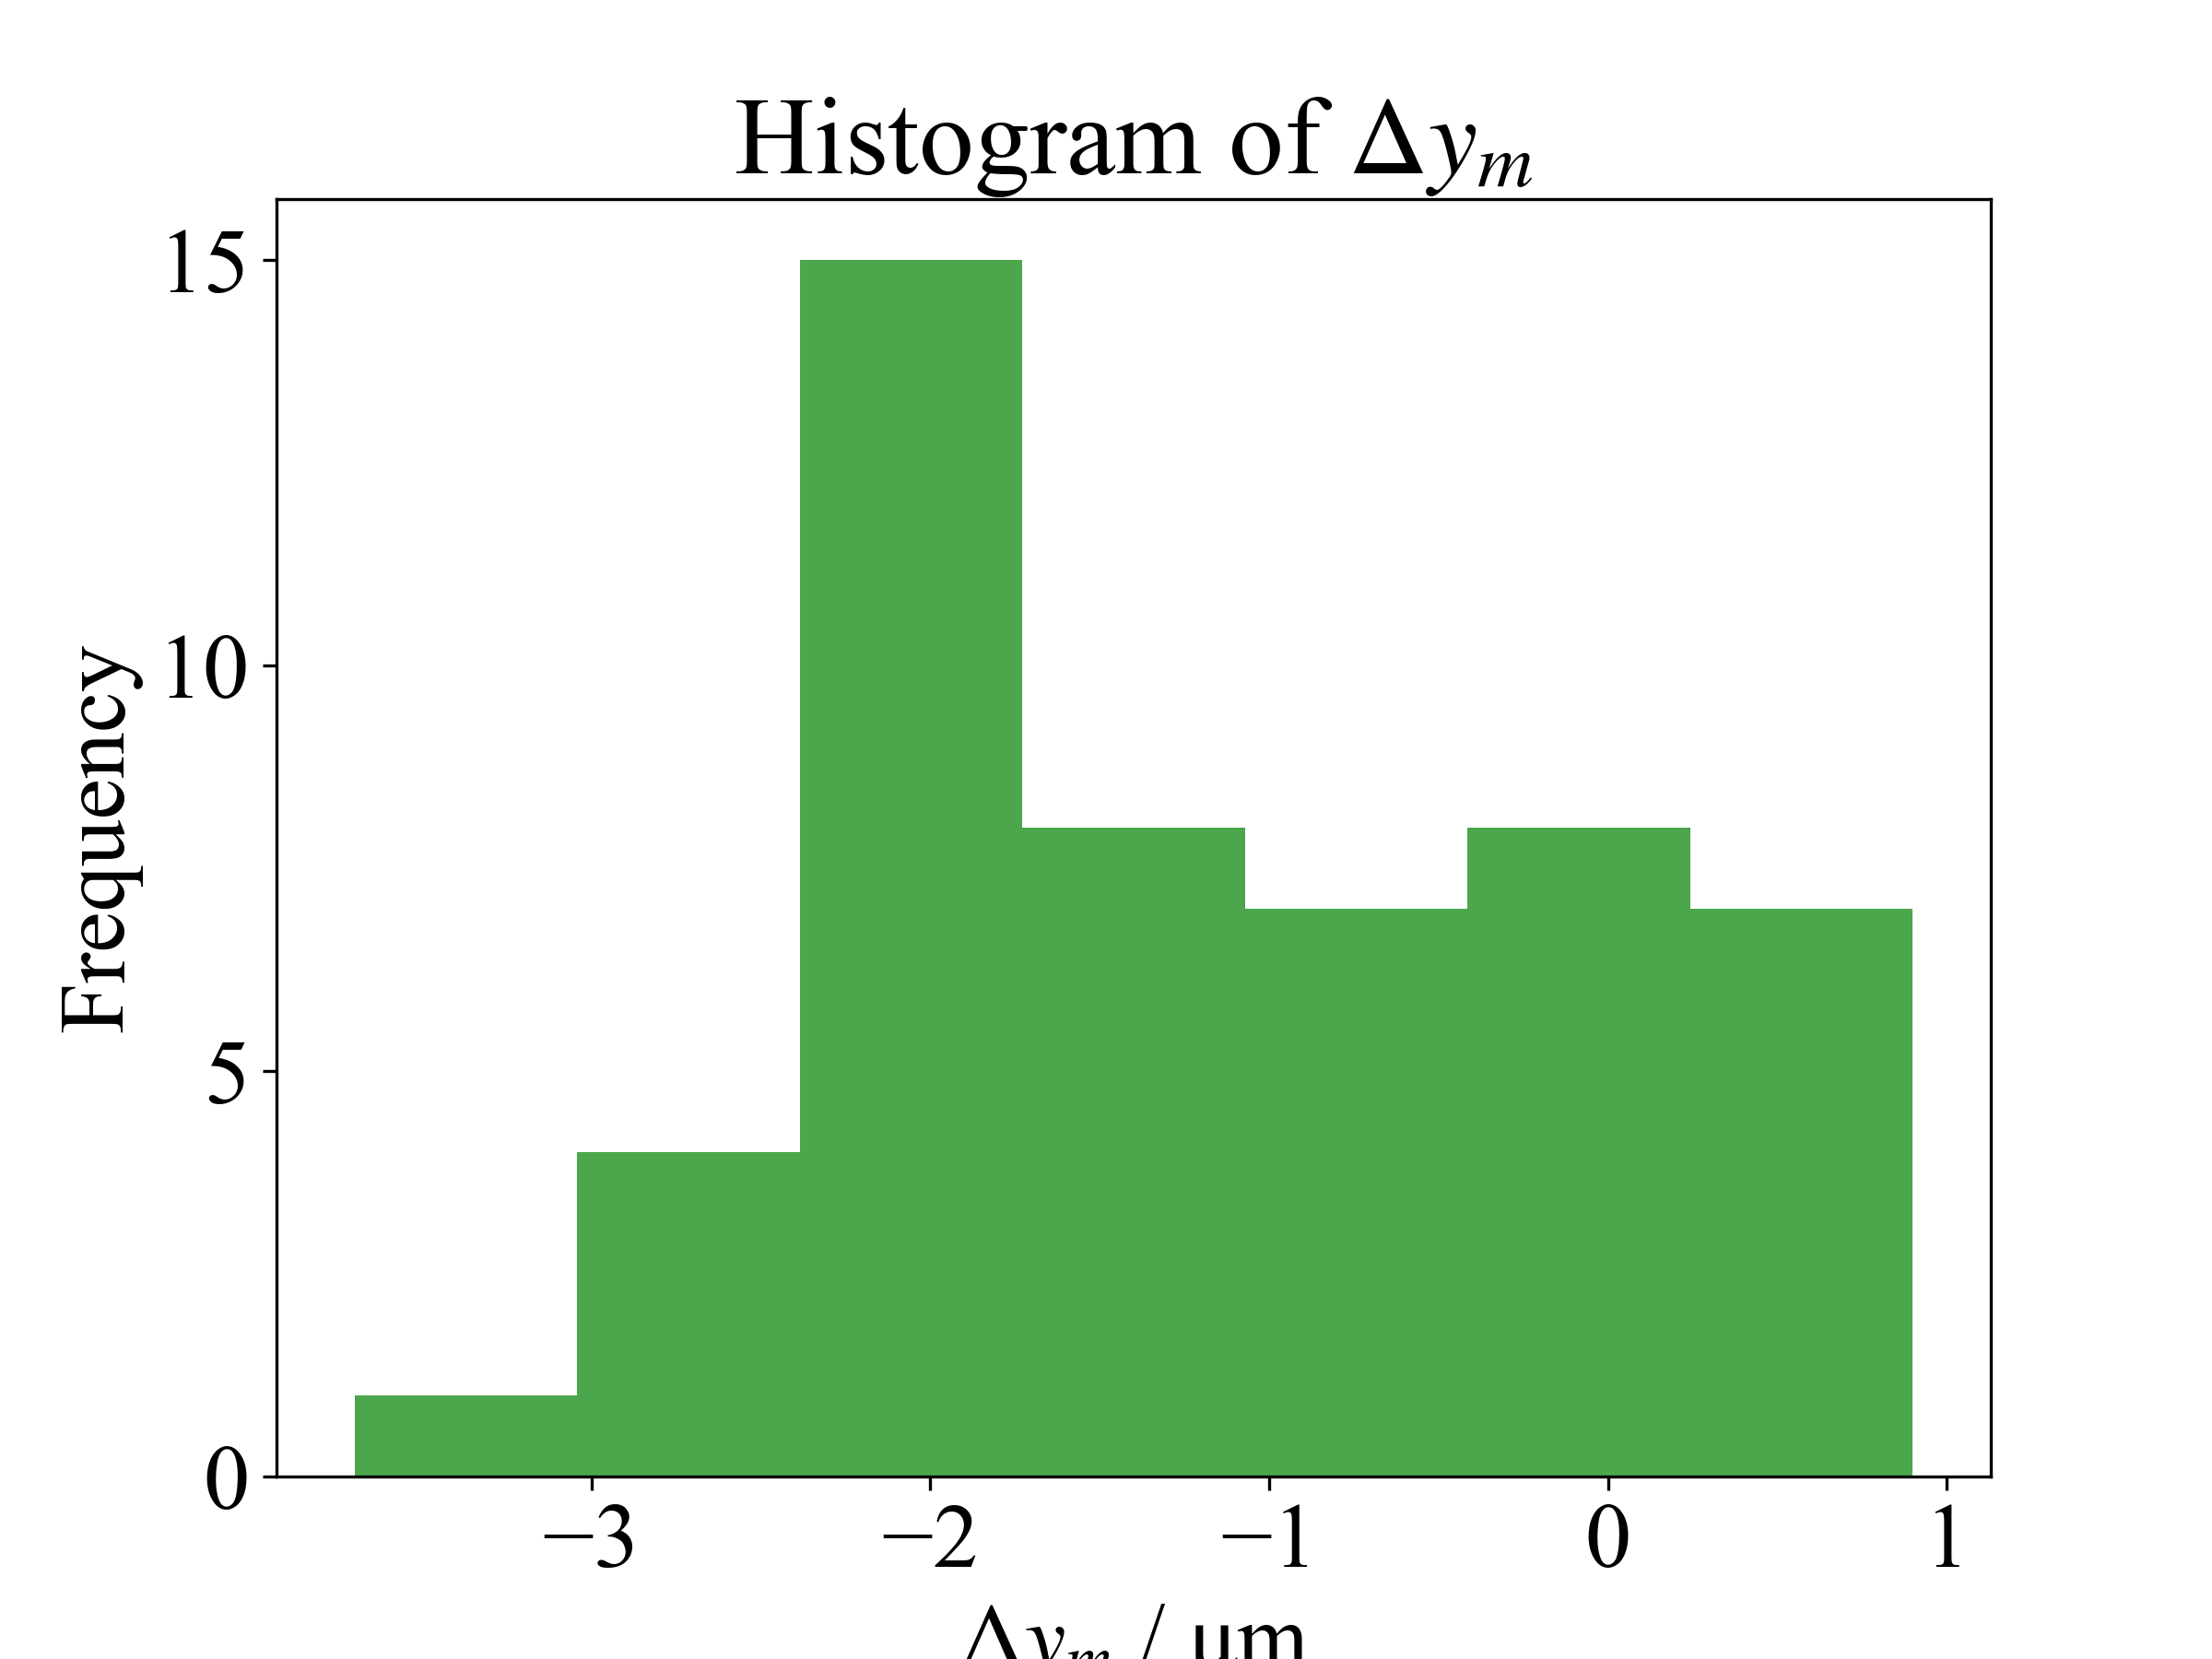
\includegraphics[width=\linewidth]{src/figures/delta-x-y-histogram/delta-y-histogram.png}
        \subcaption{$\Delta y_m$}
    \end{minipage}
    \caption{$\Delta x_m$と$\Delta y_m$のヒストグラム} \label{fig:delta-x-y-histogram}
\end{figure}

